%!TEX root = ../main.tex

\section{Prolog}
%!TEX root = ../main.tex

Wir schreiben das Jahr 1350. Hamburg wächst dank des erstarkenden Seehandels stetig und die Hanse trägt ihren Teil dazu bei. Täglich gehen am Rheinhafen Schiffe aus aller Herren Länder vor Anker, während vom Rathaus an der Troßtbrücke der Rat die Geschicke der Stadt lenkt. Es ist eine Zeit des Aufbruchs, aber auch eine Zeit der Angst. Denn neben Piraten und anderen finsteren Gestalten, die zunehmend in den Gassen der Stadt umherstreifen, greift etwas noch viel gefährlicheres um sich. Die Leute hatten bereits von einem „Schwarzen Tod" gehört, der binnen weniger Tage einen gesunden Mann seiner Lebenskraft zu berauben vermag. Nun scheint es so, als sei die Plage auch in die Wohnungen von Hamburg eingedrungen. Der düstere Geruch des Todes zieht durch die Docks und Armenviertel, während der Rat darüber entscheidet, was zu tun ist.

Und was auch immer das sein mag, es muss schnell geschehen.


\section{Kapitel 1 - Das Gespräch mit dem Rat}

%!TEX root = ../main.tex

\subsection{Das Wartezimmer}

\red{\textbf{Szene}}: Im Wartezimmer des Ratshauses

So begibt es sich, dass ihr geduldig vor einer gewaltigen Holztür im Ratshaus an der Troßtbrücke sitzt. Am gestrigen Abend wurdet ihr von Boten aufgesucht, die euch baten am folgenden Tag vor dem Hamburger Rat zu erscheinen, zu den man euch nun jeden Moment rufen wird.

Was tut ihr?

\red{\textbf{Interaktionen}}:

Die Gruppe hat noch etwas Zeit sich zu unterhalten und etwas umzusehen, bevor sie vor den Hamburger Rat gerufen werden. Sie können frei entscheiden, ob sie andere Spielcharaktere aus ihrem alltäglichen Leben bereits kennen.

\textbf{Raumbeschreibung}: Die Gruppe sitzt in einer Art Warteraum, der für damalige Verhältnisse sehr üppig eingerichtet ist. Es hängen mehrere Bilder von großen Hamburger Persönlichkeiten an den Wänden. Außerdem stehen kleine exotische Leckereien bereit, und auch Getränke werden angeboten. In einer Ecke des Raumes steht ein Ratsdiener.

An der Wand hängt eine Karte (siehe Abbildung \ref{fig:Karte}) der Stadt, welche die Charaktere sich ansehen können. Diese wird den Spielern im weiteren Verlauf des Abenteuers auch zur Verfügung stehen.

\begin{figure}[t]
	\begin{center}
		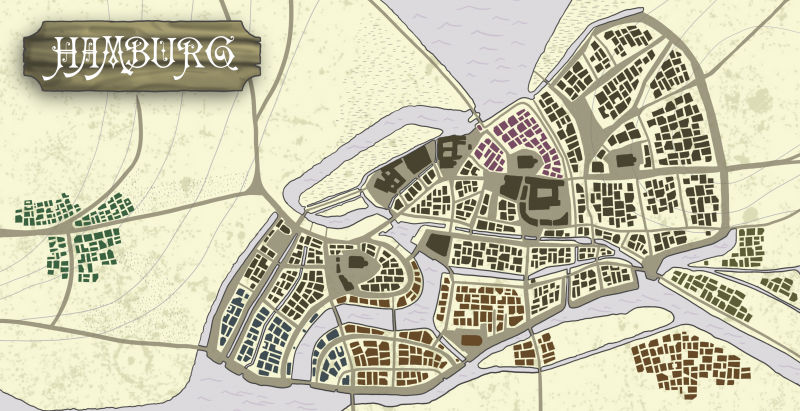
\includegraphics[scale=0.7]{./images/Karte.png}
		\caption{Stadkarte von Hamburg, anno 1350}
    \label{fig:Karte}
	\end{center}
\end{figure}


\subsection{Das Gespräch mit dem Rat}

Also Ihr euch also unterhaltet öffnet sich plötzlich die Holztür und ein junger Ratsdiener bittet euch vor den Rat zu treten.

\red{\textbf{Szene}}: Vor dem Hamburger Rat

\textbf{Raumbeschreibung}: Ihr tretet in einen großen Raum ein, der von einer U-förmigen Tischreihe dominiert werden, an dem 18 Männer in erhöhter Position sitzen. Auch wenn der Raum sonst nur spärlich eingerichtet ist, ist offensichtlich dass sich hier sonst niemand aufhält, der wenig Geld hat. Aus den Wänden sind kunstvoll Löwenköpfe und andere Muster herausgearbeitet. Eine Wand ist von hohen Fenstern gesäumt, die den Raum hell erleuchten.

Im Hintergrund huschen Ratsdiener mit Papieren umher oder gehen anderen Aufgaben nach.

\red{\textbf{Info}: Die 18 Männer setzen sich aus neun Rechtskundigen, sieben Kaufleuten und zwei Vertretern der Kirche zusammen.}

\red{\textbf{Interaktion}}:

Vorsitzender des Rates:
\gqm{\textit{Der Hamburger Rat dankt euch für euer Erscheinen. Bevor wir uns jedoch mit den euch betrauten Aufträgen befassen werden, sagt, was wisst ihr über die Pestilenz?}}

\red{\textbf{Probe auf Gesellschaft/Wissen o.Ä}: Menschen die von der Pestilenz befallen sind leiden unter Schwindelgefühlen und Schüttelfrost. Auch klagen manche über starke Kopfschmerzen und erbrechen sich häufig. Ein hohes Fieber sowie schwarze Pestbeulen an den Lymphknoten treten im Verlaufe der Krankheit auf und sind für den Patienten meist ein sicheres Todeszeichen.}

\red{\textbf{kritischer Erfolg/Probe auf Medizin}: Manche Heiler berichten, dass sie die Pestbeulen aufschneiden und vom darin enthaltenden Eiter reinigen. Wird anschließend das Fieber eines Kranken behandelt konnte mancher Totgeglaubte wieder von der Pest geheilt werden.}

Vorsitzender des Rates:
\gqm{\textit{}}


\section{Kapitel 2 - Im Sitz des Beirats}

%!TEX root = ../main.tex

\red{\textbf{Szene}}:

Nachdem ihr aus dem Rat entlassen wurdet macht ihr euch also auf den Weg zum Sitz des Beirats. In der unmittelbaren Umgebung des Ratshauses spürt man den Aufstieg Hamburgs als Handelsmetropole am deutlichsten. Ihr schlendert durch breite Straßen die von hohen Häusern gesäumt werden. Dienstboten eilen über den Pflasterstein und auch sonst herrscht geschäftiges treiben, als ihr unweit der St. Michaelis Kirche vor eine Kapelle tretet, die euch der Rat als eure Operationszentrale genannt hat

\textbf{Raumbeschreibung}: Als ihr an der kleinen Kapelle ankommt, erkennt ihr, dass es sich dabei um ein durchaus anschauliches Gebäude handelt, dass erst kürzlich einen neuen Anstrich mit weißer Farbe erhalten hat. Im Inneren stehen allerhand Tische und Stühle herum. Außerdem gibt es Schlafmöglichkeiten und so ziemlich alles, was man zum Leben so gebrauchen kann. Selbst ausgewählte Speisen stehen bereits zum Verzehr bereit.

\textbf{Ereignis}: Die Gruppe kann sich erst mal unterhalten. Ihr Gespräch wird allerdings von einem Klopfen unterbrochen ...

\begin{tcolorbox}
  Wurf: Wer oder was unterbricht das Gespräch unserer Gruppe?
  Das Militär (1 bis 33) (gehe zu \ref{militär}) \\
  Der Tod (34 bis 66) (gehe zu \ref{tot}) \\
  Ein Kind (67 bis 99) \ref{kind} \\
  Bei 100: würfle erneut.
\end{tcolorbox}

\section{Der militärische Besuch}
\label{militär}

\red{\textbf{Szene}}:

General zur Brügge steht davor und bittet um Einlass.

Gespräch mit Brügge: Dieser berichtet ihnen in vehementem Ton, dass die ganze Krise ein Werk der Dithmarscher sei. Diese hätten sich jahrelang an Hamburgs Handelsschiffen gütlich getan. Nun, da es einen Vertrag gibt, der das verhindert, versuchen einige von ihnen die Stadt zu schwächen, um davon zu profitieren oder sie gar ganz an sich zu reißen. Die Dithmarscher operieren von ihrem Versteck aus, das sich in einer Hafenkaschemme namens „Beim Gelockten Hund“ befinden soll. Ein gewisser Gorich leite das Ganze. Dort sollten sie mit ihren Recherchen beginnen.

Interaktionen:

Probe auf Menschenkenntnis:

General zur Brügge sagt schon die Wahrheit, aber seine Perspektive könnte durchaus verzerrt beziehungsweise einseitig sein.
Die Charaktere können sich aber sicher sein, dass er nicht lügt, zumindest seiner Auffassung nach nicht.

Ab hier können die Spieler frei entscheiden, wohin sie gehen wollen! Nach Ablauf der Frist von vier Tagen müssen sie beim Hamburger Rat vorsprechen. Bis dahin müssen sie sich auf eine Handlungsempfehlung festgelegt haben!


Option 2 – Der Tod
\red{\textbf{Szene}}:

Ereignis: Während sich die Gruppe noch unterhält, hören die Charaktere plötzlich ein lautes Klopfen an der Tür.

Davor steht der Totensammler Hanno. Er fragt, ob es Tote gäbe, die abzuholen seien, und ob im Haus bereits die Pest wüte.

Gespräch mit Hanno: Im Armenviertel sei es am Schlimmsten. Die Leichen könne er kaum mehr entsorgen. Man müsse kreativ werden.

Gegen Bestechung verrät er, dass er jemandem Leichen verkaufe. Dazu müsse er sie allerdings recht weit fortbringen, nämlich in einen kleinen Ort namens Eeksdurf vor den Toren der Stadt. Dort hinterlege er die leblosen Körper in einem Lagerhaus, wo bereits seine Bezahlung auf ihn warte. Die Absprache habe er dereinst mit einer jungen rothaarigen Frau getroffen.

Sie habe ihn angesprochen, nachdem sie ihn beim Abholen von Leichen im Dorf sah...


Ab hier können die Spieler frei entscheiden, wohin sie gehen wollen! Nach Ablauf der Frist von vier Tagen müssen sie beim Hamburger Rat vorsprechen. Bis dahin müssen sie sich auf eine Handlungsempfehlung festgelegt haben!


Option 3 – Ein Kind
\red{\textbf{Szene}}:

Ereignis: Es klopft plötzlich an der Tür und davor steht ein Kind zusammen mit seiner stark vermummten Mutter.

Gespräch mit der Mutter und dem Kind: Sie kämen aus dem Armenviertel Hammerbrook und seien auf der Suche nach der St. Petri-Kirche. Sie soll ein Zufluchtsort für gesunde und sündenfreie Menschen sein. Niemand werde dort krank! Für sie sei es zu spät, hustet die Frau, aber ihr kleines Kind, das sei noch zu retten. Sie wissen das alles von einem Mann, der im Armenviertel nach den Leuten sehe. Er werde nicht krank, egal was er tue ... Er habe sie losgeschickt. Sie wüssten gern den Weg.

Die Gruppe kann eine Beschreibung von Didrich von Sinnfeld erhalten. Außerdem geben ihnen die beiden auf Nachfrage den Tipp, einmal beim Lumpensammler im Armenviertel vorbeizuschauen.


Ab hier können die Spieler frei entscheiden, wohin sie gehen wollen! Nach Ablauf der Frist von vier Tagen müssen sie beim Hamburger Rat vorsprechen. Bis dahin müssen sie sich auf eine Handlungsempfehlung festgelegt haben!


\section{Kapitel 3 - Am Hafen}
\label{Hafen}
%!TEX root = ../main.tex

\red{\textbf{Szene}}:

Nach einem kurzen Fußmarsch steht ihr nun also inmitten des Hafens. Es herrscht geschäftiges Treiben. Allerlei Matrosen (\blue{\ref{Matrosen}}) und Hafenarbeiter (\blue{\ref{Hafenarbeiter}}) gehen ihren Aufgaben nach. An den Kais stehen einige Aufseher (\blue{\ref{Aufseher}}) und löschen die Ladungen der vor Anker liegenden Handelsschiffen.

\textbf{Ortsbeschreibung}: Allerhand Gesindel und unzählige Hafenarbeiter treiben sich herum. Prostituierte (\blue{\ref{Prostituierte}}) bieten ihre Dienste an, und Kinder betteln um ein wenig Brot. Hin und wieder sieht man Menschen, die sich vermummen oder gar ihr ganzes Gesicht hinter Tüchern verbergen.

\red{\textbf{Interaktionen}}:

Die Gruppe kann sich nun zum „Gelockten Hund“ aufmachen oder sich zunächst ein wenig umsehen. An den Docks treffen sie auf allerhand Charaktere, die ihnen etwas zum Hafen erzählen können.
Diese werden ihnen erzählen, dass immer mehr Arbeiter ausfallen, die mit der Lagerung von Lebensmitteln und anderen verderblichen Waren zu tun haben.

\subsection{Vor dem \gqm{Gelockte Hund}}
\label{vorhund}

\red{\textbf{Szene}}:

Ihr haltet vor einem kleinen Wirtshaus dessen besten Tage bereits weit in der Vergangenheit liegen. Es sieht - wie seine Kundschaft - ein wenig heruntergekommen aus. Vor der Türe des Gebäudes halten sich drei finstere Gestalten, bei denen es sich wohl um Seeräuber handelt, auf.

Ereignis: Schon vor der Tür wird die Gruppe unangenehm begrüßt. Die Seeräuber behaupten es würde Eintritt kosten, in den Laden zu kommen.

Es gibt nun verschiedene Möglichkeiten an den Seeräubern vorbei in das Gasthaus zu gelangen:

\begin{itemize}
  \item \red{\textbf{Probe auf Menschenkenntnis (erleichtert):} Dass der Eintritt etwas kostet, ist eine Lüge.} \\
  \item \textbf{\red{Kampf:}} Betrunkener Pirat \\
\begin{center}
  \begin{tabular}{cc}
  \toprule
  Fähigkeit & Punkte \\
  \midrule
  Leben & 80 \\
  Fäuste & 70 \\
  Schaden & 15 \\
  Parieren & 5 \\
  \bottomrule
\end{tabular}

\end{center}

Werden die Piraten besiegt können die Spieler ein verziertes Kreuz aus Silber in der Tasche eines Piraten finden.

\red{\textbf{Probe auf christliche Kultur o.ä.}: Es ist ein Kreuz, wie es sonst nur Priester tragen würden.
Auf der Rückseite ist Apostel Petrus eingraviert.}
\end{itemize}

\subsection{Im \gqm{Gelockten Hund}}
\label{imhund}

\red{\textbf{Szene}}:

Der Eindruck, dass es sich hier um eine finstere Absteige handelt bestätigt sich, als ihr eintretet. Auch das Innere dementsprechend heruntergekommen aus. Der Großteil des Publikums ist Gesindel, das Fremden gegenüber nicht sonderlich wohlgesonnen sein dürfte.

\textbf{Raumbeschreibung}: Es herrscht ausgelassene Stimmung. In der Kaschemme selbst ist erst mal aber nichts besonders ungewöhnlich.

\red{\textbf{Interaktionen}}:

Die Charaktere können sich umhören, ob jemand Gorich kennt. Sollten sie nach ihm fragen wird niemand bis auf den Wirt Gert (\blue{\ref{Gert}}) ihnen antworten.

Gert: \gqm{\textit{Edle Herren, ich würde euch gerne Auskunft geben, doch seht was hier los ist! Heute morgen ist meine Wirtin nicht zur Arbeit erschienen. Auch meine Frau, die das Essen zubereitete ist letzte Woche der Pest zum Opfer gefallen. Wenn ihr mir... ein wenig unter die Arme greifen könntet? Danach werde ich euch freilich gerne helfen!}}

Entscheidet sich die Gruppe dem Wirt Gert zu helfen, dann muss sie ihn nun bei Aufgaben in der Kneipe unterstützen. Diese Aufgaben sind:

\begin{itemize}
  \item Eintopf kochen (Probe auf Kochen o.Ä)
  \item Gäste bedienen (Probe auf Menschenkenntnis (erleichtert))
  \item Einen Streit schlichten (Probe auf Beruhigen o.Ä)
  \item Ein wenig Musizieren (Probe auf passendes Talent)
\end{itemize}

Für einen Erfolg müssen mindestens zwei der Aufgaben erfolgreich bestanden werden. Sind mehr Aufgaben erledigt kann der Wirt je nach Ermessen des Spielleiters den Abenteurern einen Schilling für ihre Dienste geben.

Schafft die Gruppe es nicht zwei der vier Aufgaben zu bewältigen gibt Gorich sich nicht zu erkennen. Er kann nur noch mit Gewalt oder Tricks dazu gebracht werden, sich zu offenbaren. Dies ist aber stark erschwert.

\red{\textbf{Szene}}:

Ein großer, bärbeißiger Mann mit schmalem Gesicht und noch schmaleren Augen tritt an euch heran. Er stellt sich als Gorich (\blue{\ref{Gorich}}) vor. Er erzählt den Abenteurern er und seine Leute haben nichts mit der ganzen Sache zu tun. Er zeigt der Gruppe sogar, dass seine eigenen Kinder im Hinterzimmer liegen... krank. Sie hatten schon früh von der Seuche gehört und auch erfahren, dass es irgendwas mit Lebensmitteln zu tun haben könnte. Denn es waren zuallererst die Bauern und Karrenlenker krank geworden, die im Umland lebten. Also kaufte er all seine Nahrung nur noch aus Einfuhr. Das schien aber auch nichts zu helfen. Denn seine Frau ist bereits gestorben, und auch seinen Kindern gehe es immer schlechter. Ein gewisser Hagen habe es ihm verkauft. Dieser lebe in Hammerbrook, direkt vor den Toren der Stadt. Gekauft habe er die Güter direkt bei einem Lagerarbeiter. Er wisse, dass auch andere, die bei ihm gekauft haben, krank wurden.

Bevor die Abenteurer aufbrechen wird Gorich sie bitten seine Kinder und ihn nicht zu verraten. Das würde den Untergang seines Geschäfts bedeuten, und dann könne er sich erst recht nicht mehr um sie kümmern.

\red{\textbf{Interaktionen}}:

\red{\textbf{Probe auf Menschenkenntnis}: Gorich scheint die Wahrheit zu sagen.}

\purple{\textbf{Pestilenz}: Jeder, der sich den Kindern von Gorich nähert, erhält Pestilenz +2.}

\green{\textbf{Moral}: Was tut die Gruppe also mit Gorich und seinen Kinder?}

Ende des relevanten Hafen-Plots. Weiter mit:

Eeksdurf (gehe zu \blue{\ref{Eeksdurf}}) \\
Hammerbrook (gehe zu \blue{\ref{Hammerbrook}}) \\
Die Kirche St. Petri (gehe zu \blue{\ref{Petri}}) \\
Der Nikolaifleet (gehe zu \blue{\ref{Fleet}}) \\


\section{Kapitel 4 - Eeksdurf}
\label{xd}
%!TEX root = ../main.tex

\subsection*{Der Weg nach Eeksdurf}
\label{nachxd}

Ihr macht euch also auf den Weg nach Eeksdurf. Schon bald drängen sich die Häuser weniger dicht und ihr verlasst Hamburg in Richtung Westen. Größtenteils verläuft der Weg aus gestampfter Erde gerade durch die Felder, an ein paar Stellen teilt sich der Weg und ihr folgt den Wegweisern nach Eeksdurf. So seid ihr also etwa eine halbe Stunde unterwegs als ihr plötzlich am Wegesrand etwas bemerkt.

\red{\textbf{Szene}}:

Im Straßengraben liegt umgekippt ein Karren. Wollen die Spieler die Szene genauer untersuchen entdecken sie, dass die Speichen der Räder gebrochen sind. Außerdem liegen im Straßengraben drei Leichen. Einer der Toten trägt ein Priestergewand und liegt mit durchgeschnittener Kehle dahingestreckt.

\red{\textbf{Probe auf Medizin o.ä.(erleichtert)}: Die anderen beiden Toten wurden durch Stichwunden in den Oberkörper getötet}

Es scheint sich um einen Raubüberfall zu handeln. Wertsachen finden sich hier keine, auch Teile ihrer Kleidung wurden den Leichen vom Leib gerissen.

\red{\textbf{Probe auf christliche Kultur o.ä. (erleichtert)}: Selbst das Kreuz, welches der Priester mit Sicherheit um den Hals trug, ist verschwunden.}

\red{\textbf{Information für den Spielleiter}: Das Kreuz kann die Gruppe an einem betrunkenen Piraten vor dem "Gelockten Hund" im Hafen finden.}

Ihr findet sonst keinen Hinweis darauf, wer die Verstorbenen sein könnte. Allerdings entdeckt ihr einige Pergamente, die in lateinischer Schrift verfasst sind.

\red{\textbf{Probe auf Latein o.ö}: Die Pergamente handeln von schwarzer Magie und anderem Volksglauben.}

Außerdem finden die Spieler bei genauerem Hinsehen in der Brusttasche des Priesters ein Brief von einem Wolfgang (\blue{\ref{Wolfgang}}) aus Eeksdurf, in dem dieser die Kirche um sofortigen Beistand in einer dringenden Sache bittet.

Ein gutes Dutzend Fußspuren führt weiter in Richtung Eeksdurf, aber auch genügend in Richtung Hamburg. Schwer zu sagen, ob sie von den Tätern oder anderen Reisenden stammen. Aber in jedem Falle sind die Spuren am Ort der Tat nicht älter als eine Stunde. Mehr ist hier nicht zu finden.

\subsection*{Ankunft in Eeksdurf}
\label{inxd}

\red{\textbf{Szene}}:

So macht ihr euch also weiter auf den Weg nach Eeksdurf. Nach einer weiteren halben Stunde seht ihr wie zwischen Bäumen die ersten Häuser des kleinen Dorfes hervortreten. Ihr folgt dem Weg und steht bald in dem kleinen Örtchen auf einer menschenleeren Straße. Durch den alltäglichen Klatsch und Tratsch wisst ihr, dass die meisten Einwohner hier einfache Handwerker und Bauern sind. Vom sonst so geschäftigen Treiben ist nun nichts mehr zu spüren, es ist alles verlassen. Türen und Fenster sind verrammelt.

Klopfen die Spieler an eine der Türen, dann antwortet man ihnen, wenn sie passend würfeln.

\begin{tcolorbox}
  Wurf: Wird ihnen auf das Klopfen geantwortet? \\
  0 bis 49: Ihnen wird geantwortet. \\
  50 bis 99: Ihr Klopfen bleibt unbeantwortet.\\
\end{tcolorbox}

Sollte einer der Dorfbewohner mit ihnen sprechen macht er einen verängstigten Eindruck. Wo die anderen alle seien wisse er nicht.

\red{\textbf{Probe auf Menschenkenntnis}: Das er nicht wisse wo alle seien ist eine Lüge.}

Fragen die Spieler nach einer rothaarigen Frau erzählt man ihnen von Ruth (\blue{\ref{Ruth}}), der Tochter der Kräutersammlerin Ottilde (\blue{\ref{Ottilde}}). Diese wohne gleich die Straße runter am Dorfesrand in einer kleinen verfallenen Hütte. Wenn man der Straße folge könne man es nicht verfehlen.

\red{\textbf{Probe auf Menschenkenntnis}: Auch die Wegweisung ist eine Lüge.}

Folgen die Spieler diesem Weg gelangen sie bald an den Dorfesrand, dort ist nirgends ein Haus zu sehen, das auf die Beschreibung des Dorfbewohners passt. Jedoch hören die Abenteurer ein Geräusch...

\begin{tcolorbox}
  Wurf: Was hört die Gruppe? \\
  1 bis 50: Sie hören aufgebrachte Stimmen. (gehe zu \blue{\ref{mob}})\\
  51 bis 100: Sie hören ein Knacken und Rauschen. (gehe zu \blue{\ref{feuer}})\\
\end{tcolorbox}

\subsubsection*{Option 1 - Der wütende Mob}
\label{mob}

\red{\textbf{Szene}}:

Ihr folgt den Geräuschen und gelangt an eine kleine Hütte vor dem Waldrand. Die Hütte macht einen verfallenen Eindruck, scheint aber noch bewohnt zu sein. Vor der Haustüre stehen wütend grölende Menschen und schwingen Mistforken, während eine alte, merkwürdig gekleidete Dame vor der Hütte versucht sie zu besänftigen.
Aus den aufgebrachten Wortgefechten lässt sich schließen, dass es sich bei der Dame um die Kräuterfrau Ottilde handelt.

Der Rädelsführer des Mobs ist ein Bauer namens Wolfgang (\blue{\ref{Wolfgang}}). Dieser fordert vehement, dass Ruth aus dem Haus herauskommt. Sie sei an dem Unglück Schuld! Schwarze Magie habe sie angewandt und nicht mal die Kirche wolle den Bewohnern mehr helfen, obwohl man mit einem Brief um Hilfe gebeten hatte!

\red{\textbf{Interaktionen}}:

Die Gruppe sollte versuchen den wütenden Mob zu beruhigen. Im Gespräch werden die Leute im Mob sich immer wieder auf vier Argumente berufen:

\begin{itemize}
  \item Ruth soll wiederholt dabei gesehen worden sein, wie sie nachts tote Körper in die große Scheune gebracht habe.
  \item Ruth habe den Brief an die Kirche, welchen sie dem Totensammler mitgeben sollte, nie übergeben.
  \item Ruth habe die Pest gebracht. Sie war in Hamburg gewesen, um Korn zu kaufen.
  \item Kaum war sie zurück, brach die Krankheit aus! Zu diesem Zeitpunkt sei noch nirgends sonst in der Gegend jemand erkrankt!
\end{itemize}

\red{\textbf{Probe auf Beruhigen}}:

\begin{itemize}
  \item Erfolg \\
  Schaffen Sie es den Mob zu beruhigen, dann zieht sich der Mob zurück und sie können mit Ottilde in Ruhe das Haus betreten. Dort treffen sie auch auf Ruth, die verängstigt in einer Ecke sitzt.
  \item Misserfolg \\
  Schaffen sie es nicht den Mob zu beruhigen, dann bricht dieser in das Haus ein. Wollen die Abenteurer den Mob hindern kommt es zum Kampf (\blue{\ref{kampf}}) mit Bauern. Im Haus fehlt jedenfalls so oder so jede Spur von Ruth. Ottilde ist dankbar für ihre Hilfe und verrät der Gruppe, dass Ruth sich in der großen Scheune verstecke.
\end{itemize}

Ruth wird der Gruppe kleinlaut erzählen, dass sie nichts gemacht habe und nicht wisse warum die Bauern so aufgebracht seien

\red{\textbf{Probe auf Menschenkenntnis}}:

Ruth lügt. Hakt die Gruppe nach, dann erzählt sie, ihnen die gesamte Geschichte. \\
Sie habe direkt am Nikolaifleet Korn holen wollen. Da sei es am günstigsten, habe man ihr gesagt. Als sie dort ankam, sei es bereits spät gewesen. Sie habe am Lagerhaus, das man ihr beschrieben hatte, angeklopft, allerdings ohne Erfolg. Also habe sie durchs Fenster geschaut und einen Mann erblickt, der sich über etwas gebeugt habe. Er soll eine Art Vogel-Maske und einen weiten Mantel getragen haben. Ruth sagt, sie habe Angst gehabt und habe davonlaufen wollen. Sie sei auf dem Schnee ausgerutscht und habe das Gleichgewicht verloren. Dabei sei mit dem Kopf aufgeschlagen und im Lagerhaus wieder zu sich gekommen. Der Mann habe sich ihr dann als Didrich vorgestellt. Er forsche an der Pestilenz, habe er erklärt. Nur darum sei er so gekleidet und habe sich an der Leiche zu schaffen gemacht. Ruth habe ihm dann erzählt, dass in Eeksdurf zwar niemand krank sei, aber dass der Totensammler regelmäßig mit den Leichen durch ihr Dorf fahre, um diese tief im Eekshult zu verscharren. Daraufhin habe Didrich ihr einen Handel vorgeschlagen, und... naja... Ruth habe angenommen. \gqm{\textit{Wieso auch nicht. Die sind schließlich tot und ich arm. Eins davon kann man wenigstens noch ändern.}}
Die Leichen habe sie also von da an immer in ein kleines Lagerhaus im Armenviertel Hammerbrook gebracht. Dort habe auch ihr Geld gelegen...

Sollte die Gruppe nachfragen, kann Ruth ihnen genau sagen, in welchem Lagerhaus sie die Leichen ablegt.

\subsubsection*{Option 2 – Ein großes Feuer}
\label{feuer}

\red{\textbf{Szene}}:

Ihr folgt den Geräuschen und gelangt an eine kleine Hütte vor dem Waldrand. Die Hütte macht einen verfallenen Eindruck, scheint aber noch bewohnt zu sein. Es ist weit und breit niemand zu sehen, vor der offenen Tür der Hütte seht ihr jedoch ein gewaltiges Feuer. Im Feuer zeichnen sich die verkohlten Überreste zweier Menschen ab.

Die Gruppe kann wenn gewünscht die Hütte betreten.

\textbf{Raumbeschreibung}: Das Innere der Hütte macht genauso wenig her wie die Fassade vermuten lässt. In einer Ecke des einzigen Raumes ist Stroh auf dem Boden ausgebettet. Ein morscher Holztisch und zwei Stühle stehen in der anderen Ecke. Das einzige herausstechende im Raum ist ein Regal, dass eine ganze Wand einnimmt, und auf dem getrocknete Kräuter säuberlich aufgereiht sind.

Bei genauerem Hinsehen findet die Gruppe ein Blatt Pergament, auf dem eine Art Wegbeschreibung gekritzelt zu sein scheint - nur sehr grob. Der Weg führt zu einem Ort im Armenviertel Hammerbrook, mehr lässt die Karte nicht erkennen. Außerdem finden die Abenteurer Geld. Etwas mehr Geld als jemand der hier lebt besitzen sollte.

Beim Verlassen der Hütte trifft die Gruppe auf Wolfgang (\blue{\ref{Wolfgang}}) und Hermann (\blue{\ref{Hermann}}). Diese werfen ihnen umgehend vor, mit der bösen Zauberin im Bunde zu sein und werden sie angreifen (gehe zu \blue{\ref{kampf}}) falls die Gruppe nicht schafft die beiden zu beruhigen.

\red{\textbf{Probe auf Beruhigen o.ä}: Die Bauern erzählen, weshalb sie Otthilde und Ruth verbrannt haben}

\begin{itemize}
  \item Ruth soll wiederholt dabei gesehen worden sein, wie sie nachts tote Körper in die große Scheune gebracht habe.
  \item Ruth habe den Brief an die Kirche, welchen sie dem Totensammler mitgeben sollte, nie übergeben.
  \item Ruth habe die Pest gebracht. Sie war in Hamburg gewesen, um Korn zu kaufen.
  \item Kaum war sie zurück, brach die Krankheit aus! Zu diesem Zeitpunkt sei noch nirgends sonst in der Gegend jemand erkrankt!
\end{itemize}

\subsubsection*{Kampf gegen die Bauern}
\label{kampf}

\begin{center}
  \begin{tabular}{lcc}

    \toprule
    Fähigkeit & \textbf{Wolfgang} & \textbf{Hermann} \\
    \midrule
    Leben & 70 & 70 \\
    Waffe & Fäuste (70) & Mistgabel (70) \\
    Schaden & 15 & 40 \\
    Parieren & 5 & 30 \\
    \bottomrule
  \end{tabular}
\end{center}



\violet{\textbf{Moral}: Wie reagiert unsere Gruppe auf die Situation in Eeksdurf?}

Ende des relevanten Eeksdurf-Plots.

Hafen (gehe zu \blue{\ref{Hafen}}) \\
Hammerbrook (gehe zu \blue{\ref{arm}}) \\
Die Kirche St. Petri (gehe zu \blue{\ref{Petri}}) \\
Der Nikolaifleet (gehe zu \blue{\ref{Fleet}}) \\

